\section{Git}
Ein VCS (Version-Control System) ist ein System, das zur Erfassung von Änderungen an Dokumenten oder Dateien verwendet wird. Alle Versionen werden in einem Archiv mit Zeitstempel und Benutzerkennung gesichert und können später wiederhergestellt werden. Ein verbreitetes VCS ist in der Software Enwicklung \textbf{Git}.

\subsection{Git Übersicht - Vereinfacht}
In einem Git-Repository (aka. Git Projekt) hat jede Datei eines der drei Zustände.\\
\begin{center}
	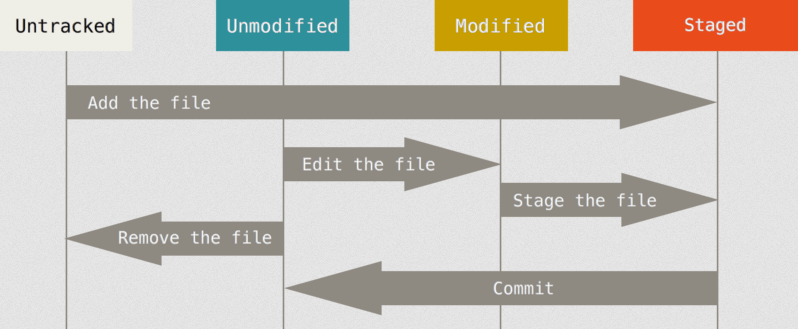
\includegraphics[width=\columnwidth]{Images/git.png}
\end{center}
\begin{tabular}{p{9cm}}
	\textbf{Untracked}, Datei wird von git irgnoriert \\
	\textbf{Unmodified}, Datei ist nicht bearbeitt worden (in git gesichert)\\
	\textbf{Modified}, Datei ist bearbeitet wird aber nicht gesichert\\
	\textbf{Staged}, Datei ist bearbeitet und wird beim nächsten Commit gesichert
\end{tabular}
~\\~\\
Um Änderungen von Dateien in git zu Speichern, müssen diese als staged eingetragen sein. Beim Speichern wird ein \textbf{Commit} erstellt und dem letzten Commit hinzugefügt. Dadurch entsteht eine Liste von Änderungen aka. History. Zu jedem Commit kann gesprungen werden, und neue Commits hinzugefügt werden. Dadruch entsteht \textbf{Branches}, welcher unabhängig von anderen verändert werden können. Der \textbf{HEAD} zeigt immer auf den aktiven Commit.
\begin{center}
	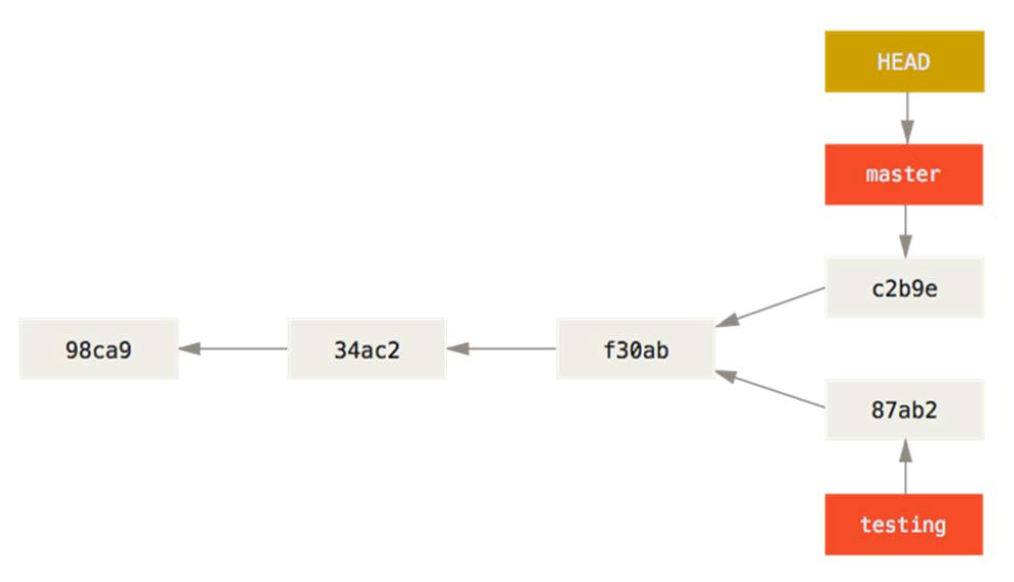
\includegraphics[width=\columnwidth]{Images/branches}
\end{center}


Commits können an eine anders Git-Repository auf zB einem Server (im folgenden als \textbf{Remote} bezeichnet) geschickt bzw heruntergeladen werden.
\begin{center}
	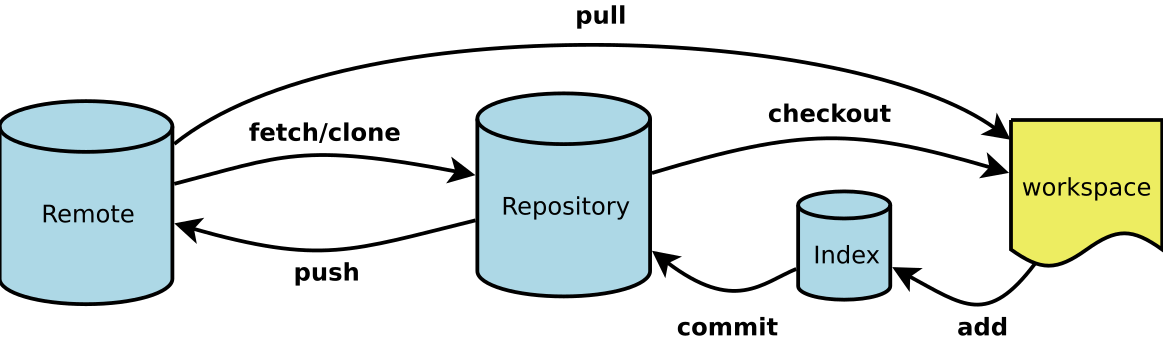
\includegraphics[width=\columnwidth]{Images/remote}
\end{center}

